\documentclass[a4paper,12pt]{article}
\usepackage[top = 2.5cm, bottom = 2.5cm, left = 2.5cm, right = 2.5cm]{geometry}
% Unfortunately, LaTeX has a hard time interpreting German Umlaute. The following two lines and packages should help. If it doesn't work for you please let me know.
\usepackage[T1]{fontenc}
\usepackage[utf8]{inputenc}
% The following two packages - multirow and booktabs - are needed to create nice looking tables.
\usepackage{multirow} % Multirow is for tables with multiple rows within one cell.
\usepackage{booktabs} % For even nicer tables.
% As we usually want to include some plots (.pdf files) we need a package for that.
\usepackage{graphicx}
\usepackage{tikz}
% The default setting of LaTeX is to indent new paragraphs. This is useful for articles. But not really nice for homework problem sets. The following command sets the indent to 0.
\usepackage[spanish]{babel}
\usepackage{setspace}
\setlength{\parindent}{0in}
% Package to place figures where you want them.
\usepackage{float}
% The fancyhdr package let's us create nice headers.
\usepackage{fancyhdr}
\usepackage{amsmath}
\usepackage{amssymb}
\usepackage{natbib}
\usepackage{apalike}
\usepackage{graphicx}
\usepackage{subcaption}
\usepackage{booktabs}
\usepackage{etoolbox}
\usepackage{amsthm}
\AtBeginEnvironment{align}{\setcounter{equation}{0}}
\newenvironment{solution}
  {\renewcommand\qedsymbol{$\blacksquare$}\begin{proof}[Solución]}
  {\end{proof}}
\pagestyle{fancy}

\fancyhf{}

\lhead{\footnotesize Tarea 2}
\rhead{\footnotesize  Rompich}
\cfoot{\footnotesize \thepage}



\begin{document}
    \thispagestyle{empty} % This command disables the header on the first page.

    \begin{tabular}{p{15.5cm}} % This is a simple tabular environment to align your text nicely
    \begin{tabbing}
    Universidad del Valle de Guatemala 
    \\
    Departamento de Matemática\\ Licenciatura en Matemática Aplicada \\ Fecha de entrega: 26 de febrero de 2021  \\
    Rudik R. Rompich   - Carné: 19857\\
    \end{tabbing}
    Estadística 2 - Eugenio Aristondo \\
    \hline % \hline produces horizontal lines.
    \\
    \end{tabular} % Our tabular environment ends here.
    \vspace*{0.3cm} % Now we want to add some vertical space in between the line and our title.
    \begin{center} % Everything within the center environment is centered.
    {\Large \bf Tarea 2
} % <---- Don't forget to put in the right number
        \vspace{2mm}
    \end{center}
    \vspace{0.4cm}


\section{Capítulo 13}
\subsection{Ejercicio 1}
\begin{center}
    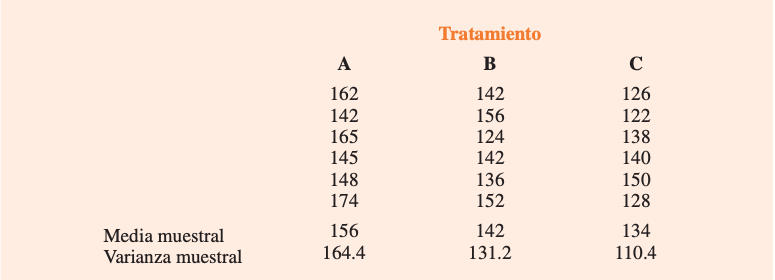
\includegraphics[scale=0.5]{Imagenes/1.png}
\end{center}
\begin{enumerate}
    \item  Calcule la suma de cuadrados entre tratamientos.
    \begin{solution}
    \begin{align}
        \intertext{Se sabe que: }
        SCTR &= \sum_{j=1}^k n_j(\Bar{x}_j-\Bar{\Bar{x}})^2\\
             &= 6\left[(156-144)^2+(142-144)^2+(134-144)^2\right]\\
             &= 1488
    \end{align}
    \end{solution}
    \item  Calcule el cuadrado medio entre tratamientos
    \begin{solution}
    \begin{align}
        \intertext{Considerando a $k$ como el número de grupos:}
        CMTR &= \frac{SCTR}{k-1}\\
             &= \frac{1488}{3-1}\\
             &= \frac{1488}{2}\\
             &= 744
    \end{align}
    \end{solution}
    \item  Determine la suma de cuadrados debido al error.
    \begin{solution}
    \begin{align}
        \intertext{Considerando $s_j^2$ como la varianza, entonces:}
        SCE &= \sum_{j=1}^k (n_j-1)s_j^2\\
            &= (6-1)[164,4+131,2+110,4]\\
            &= 2030
    \end{align}
    \end{solution}
    \item  Calcule el cuadrado medio debido al error.
    \begin{solution}
    \begin{align}
        CME &= \frac{SCE}{n_T-k}\\
            &= \frac{2030}{18-3}=135.3\Bar{3}
    \end{align}
    \end{solution}
    \item  Establezca la tabla ANOVA para este problema.
    \begin{solution}
    Considerando la solución de Excel: 
    \begin{center}
        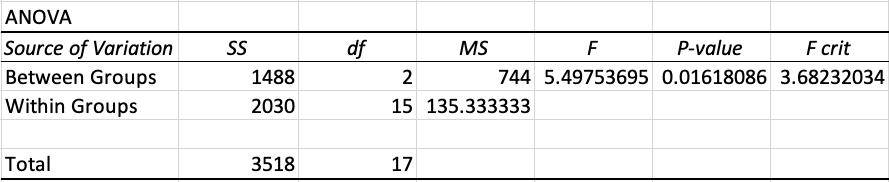
\includegraphics[scale=.4]{Imagenes/1.1.png}
    \end{center}
    \end{solution}
    \item  Con $\alpha=0.05$, pruebe si las medias de los tres tratamientos son iguales.
    \begin{solution}
    \begin{align}
        F&= \frac{CMTR}{CME}=\frac{744}{135,3\Bar{3}}=5,498
    \intertext{Considerando los grados de libertad:}
    \text{g.l.d} &= n_T-k =18-3 =15\\
    \text{g.l.n} &= k-1 = 3-1=2\\
    \intertext{Tomando como referencia la tabla B de distribución F de la página 986 del libro de texto, tenemos:}
    F&=3,68
    \end{align}
    Por lo tanto, se rechaza la $H_0$ ya que $F>F_\alpha$. Las medias no son iguales.
    \end{solution}
\end{enumerate}
\subsection{Ejercicio 2}
En un diseño completamente aleatorizado, para cada uno de los cinco niveles del factor se usaron siete unidades experimentales. Complete la tabla ANOVA siguiente.
    \begin{center}
    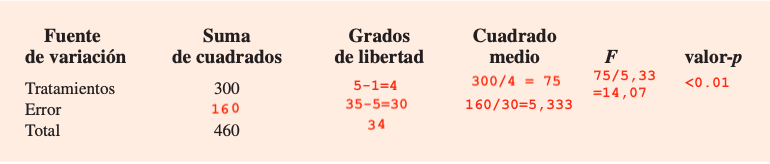
\includegraphics[scale=0.5]{Imagenes/2.png}
\end{center}
\subsection{Ejercicio 7}
 Un ingeniero propone tres métodos distintos para ensamblar un producto. Para determinar el número de unidades ensambladas correctamente con cada método, se selecciona al azar a 30 empleados y se asignan de manera aleatoria a los tres enfoques propuestos, de manera que cada método sea empleado por 10 trabajadores. Se anota el número de unidades producidas correctamente y a estos datos se les aplica el análisis de varianza. Los resultados son los siguientes: STC= 10 800; SCTR = 4560.
 
 \begin{enumerate}
     \item Establezca la tabla ANOVA de este problema.
     \begin{solution}
     \begin{center}
         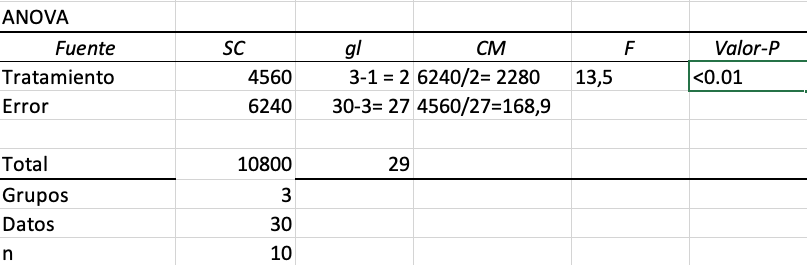
\includegraphics[scale=.5]{Imagenes/3.png}
     \end{center}
     \end{solution}
     \item  Use $\alpha =0.05$ para determinar si existen diferencias significativas entre las medias de los tres métodos de ensamble.
     \begin{solution}
     Se determinó que el Valor-P es $<0.01$ por lo cual se rechaza $H_0$ y se termina que las medias no son iguales.
     \end{solution}
 \end{enumerate}
\subsection{Ejercicio 10}
En una auditoría, los auditores tienen que emitir opiniones acerca de diversos aspectos con base en sus propias experiencias directas (Direct), indirectas (Indirect) o la combinación (Combination) de ambas. En un estudio se pidió a los auditores que dieran su opinión acerca de la frecuencia con que se presentan errores en una auditoría. Luego se compararon estas opiniones con los resultados reales. Suponga que los resultados que se presentan a continuación se obtu- vieron de un estudio similar; los valores bajos indican opiniones más acertadas.
\begin{solution}
Considerando: 
\begin{center}
    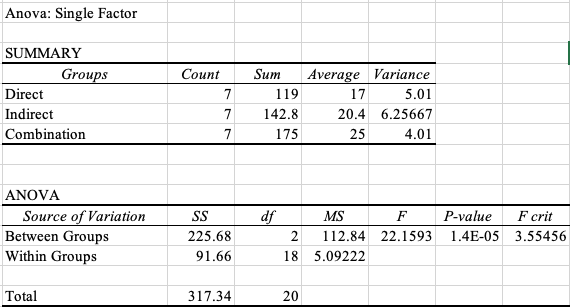
\includegraphics[scale=0.5]{Imagenes/10.png}
\end{center}
Se puede determinar por la prueba del valor-P que $1.4E-05 < \alpha =0.05$. Por lo tanto, se rechaza la $H_0$, diciendo que las medias no son iguales. Es decir el tipo de experiencia en que se basa la opinión afecta no afecta su calidad.
\end{solution}
\subsection{Ejercicio 12}
La Encuesta de satisfacción de clientes de restaurantes de Consumer Reports se basa en más de 148599 visitas a diferentes cadenas de restaurantes de servicio completo (sitio web de Consumer Reports). Una de las variables en el estudio es el precio de los alimentos, la cantidad promedio que paga una persona por la comida y la bebida, menos la propina. Suponga que un reportero del Sun Coast Times cree que sería de interés para sus lectores realizar un estudio similar en los restaurantes ubicados en la zona del Grand Strand en Myrtle Beach, Carolina del Sur. El reportero seleccionó una muestra de ocho restaurantes de mariscos (Seafood) ocho italianos (Italian) y ocho de carnes (Steakhouse). Los datos a continuación muestran los precios de la comida en dólares de los 24 negocios muestreados. Utilice $\alpha= 0.05$ para probar si hay una diferencia significativa entre el precio medio de la comida en los tres tipos de restaurantes.
\begin{solution}
Considerando: 
\begin{center}
    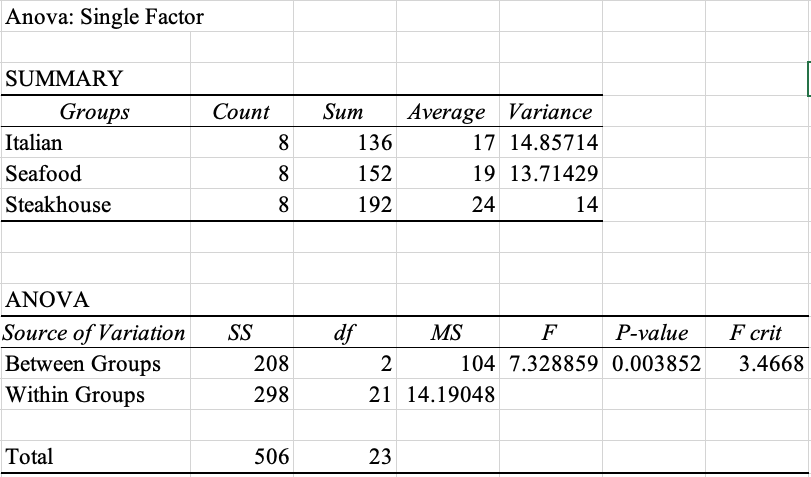
\includegraphics[scale=0.5]{Imagenes/12.png}
\end{center}
Por lo tanto, por la prueba del valor-p se rechaza la $H_0$ ya que $0.003852<\alpha=0.05$. Esto, quiere decir que sí hay una diferencia significativa en el precio medio de la comida.
\end{solution}
\subsection{Ejercicio 15}
Con el fin de probar si la media del tiempo necesario para mezclar un lote de un material es la misma si emplea las máquinas de tres fabricantes, Jacobs Chemical obtiene los datos siguientes sobre el tiempo (en minutos) requerido para mezclar el material.
\begin{enumerate}
\item Use estos datos para probar si las medias poblacionales de los tiempos necesarios para mezclar un lote de material usando las máquinas de estos tres fabricantes difieren. Use $\alpha= 0.05$.
\begin{solution}
Considerando: 
\begin{center}
    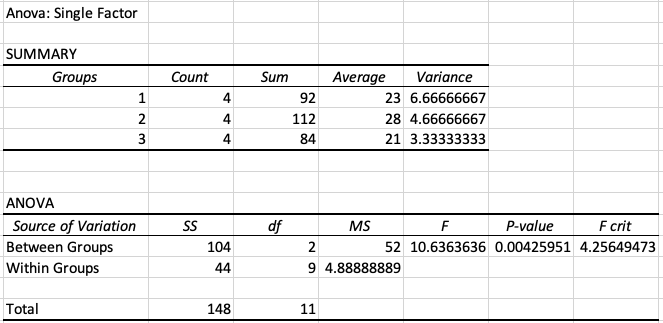
\includegraphics[scale=0.5]{Imagenes/15.png}
\end{center}
Por medio de la prueba F, se rechaza la $H_0$ ya que $F>F_\alpha$. Es decir, las medias no son iguales, es decir que las medias para mezclar un lote de material difieren.
\end{solution}
\item Con $\alpha=0.05$ como nivel de significancia, use el procedimiento LSD de Fisher para probar la igualdad entre las medias obtenidas con las máquinas del fabricante 1 y del fabricante 3. ¿Qué conclusión se obtiene después de realizar la prueba?
\begin{solution}
Considerando: \begin{center}
    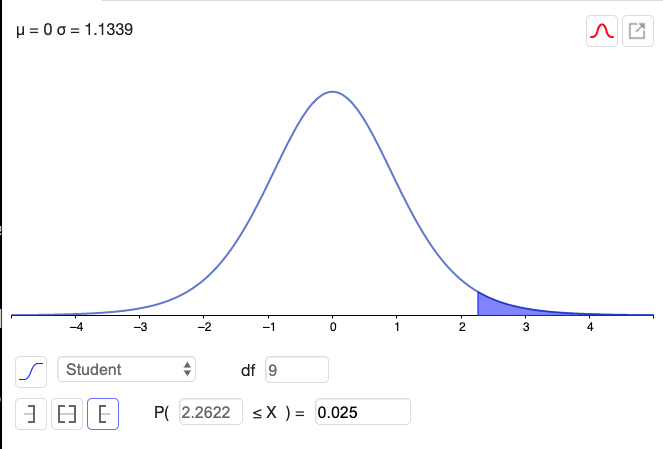
\includegraphics[scale=0.5]{Imagenes/15-2.png}
\end{center}
\begin{align}
    \intertext{Para calcular el LSD:}
    LSD &= t_{\alpha/2}\sqrt{CME\left(\frac{1}{n_i}+\frac{1}{n_j}\right)}\\
        &= t_{0.025}\sqrt{4.88889\left(\frac{1}{4}+\frac{1}{4}\right )}\\
        &= 2.2622\sqrt{4.88889\left(\frac{2}{4}\right )}\\
        &= 3.5366
    \intertext{Entonces, tenemos tres casos:}
    |x_1-x_2| &= |23-28| = 5 > LSD \text{ se rechaza $H_0$}\\
    |x_1-x_3| &= |23-21| = 2 < LSD \text{ no se rechaza $H_0$}\\
    |x_2-x_3| &= |28-21| = 7 > LSD \text{ se rechaza $H_0$}\\
\end{align}
Esto, quiere decir que entre 1 y 3 no hay una diferencia significativa. Mientras que 1 con 2 y 2 con 3 sí existe una diferencia.
\end{solution}
\end{enumerate}
\subsection{Ejercicio 18}
Para probar si existe una diferencia significativa entre cuatro máquinas respecto del número de horas entre dos averías, se obtuvieron los datos siguientes.

\begin{enumerate}
    \item Con $\alpha =0.05$, como nivel de significancia, ¿cuál es la diferencia, si hay alguna, entre las medias poblacionales de los tiempos de las cuatro máquinas?
    \begin{solution}
    Considerando:
    \begin{center}
        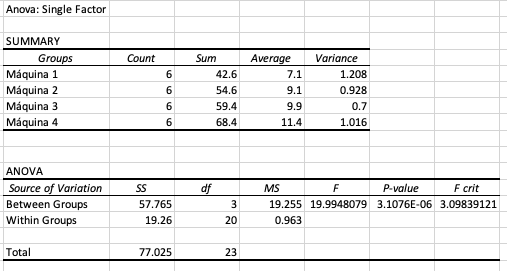
\includegraphics[scale=0.7]{Imagenes/18.png}
    \end{center}
    Por medio de la prueba F, se rechaza la $H_0$ ya que $F>F_\alpha$. Es decir, las medias no son iguales, es decir que las medias para mezclar un lote de material difieren.
    \end{solution}
    
    \item  Use el procedimiento LSD de Fisher para probar la igualdad de las medias en las máquinas 2 y 4. Utilice 0.05 como nivel de significancia.
    \begin{solution}
    Considerando: 
\begin{center}
    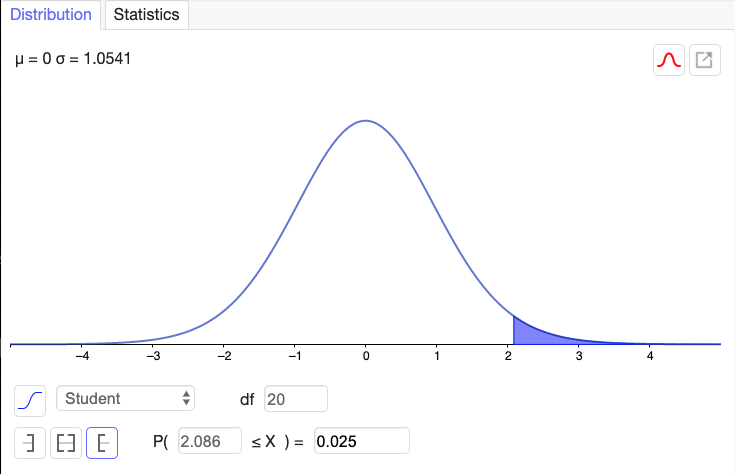
\includegraphics[scale=0.5]{Imagenes/18-1.png}
\end{center}
\begin{align}
    \intertext{Sabemos que:}
     LSD &= t_{\alpha/2}\sqrt{CME\left(\frac{1}{n_i}+\frac{1}{n_j}\right)}\\
         &= t_{0.025}\sqrt{0,963\left(\frac{1}{6}+\frac{1}{6}\right)}\\
         &= 2,086\sqrt{0,963\left(\frac{2}{6}\right)}\\
         &= 1,1819
    \intertext{Entonces, haciendo el test:}
    |x_2-x_4| &= |(9,1)-(11,4)| \\
              &= 2.3 \text{ Se rechaza $H_0$, ya que $|x_2-x_4|> LSD$} 
\end{align}
    En conclusión, sí existe una diferencia significativa.
    \end{solution}
\end{enumerate}


\end{document}